\chapter{Qca Overview}\label{sec:qca}

Quantum Dot Cellular Automata (QCA) are a quantum extension to the classical notion of Cellular Automata. 

In computability theory, we identify a Cellular Automata (CA) as a Turing-complete abstract machine model consisting of a grid of \textsl{cells} each of which can be in any of a finite number of \textsl{states}. For every cell in the grid, moreover, we define its \textsl{neighborhood}, which is the set of "near enough" cells. The \textsl{evolution} of this automaton is defined by the transition of the state of the cells, which is a function of both the status of the cell and the status of its neighborhood.

What makes a QCA different from a classical CA is that its physical implementation is regulated by the quantum laws of physics instead of the classical ones. Let's take a closer look to a QCA. As you can see in \figurename~\ref{fig:qca} a QCA is made of three main components: electron wells, crystalline substrate and electrons. Here we depict the charge of the electrons on the wells/dots by blurred blue clouds instead of the more classical representation of small, crisply defined points. This is accurate because the Quantum Mechanics says that at this near atomic scale, charge (on electrons and protons) does not come in sharp little balls, but instead is correctly representable only in a probabilistic way via the wave function (Schr\"{o}dinger equation).

\begin{figure}[h!bt]
	\centerline{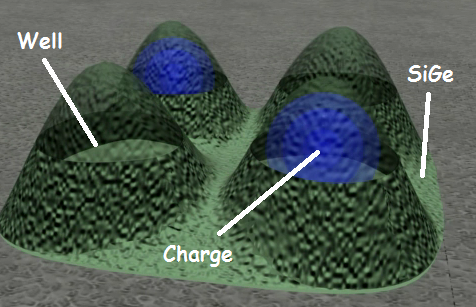
\includegraphics[width=0.8\textwidth]{img/qca.png}}
	\caption{A single Quantum Dot Cellular Automata (QCA) cell. In green the crystalline (SiGe - Silicon Germanium) substrate, where are clearly visible, in squared position, the four wells meant for accomodating that many electrons. Even though different configurations of the dots are possible, this is by far the most commonly studied structure. The blue cloud represents the amplitude of probability of finding an electron in that position.}
	\label{fig:qca}
\end{figure}

Charges of the same type (positive or negative) still repel one another so our two clouds of charge will move as far from the another as possible by moving to opposite corners of the QCA (this allows for the largest distance to be set between the clouds). In \figurename~\ref{fig:qcaevo} is represented the typical evolution of a QCA cell. It is quite easy to generalize the represented mechanism to a situation where an arbitrarily large number of cells are put adjacently in order to form, for example, a so called \textsl{quantum wire}. In such a configuration, whenever a cell switches from a state to the opposite, so does its neighbour and the neighbour of the neighbour... and so on until the end of the wire. This mechanism allows for information to be \textsl{transmitted}.

But what is the phenomenon that allows a charge to move precisely from a well to the other? This is called ''tunnel effect'' and it is a well known phenomenon in quantum physics stating that, under certain hypothesis, waves (in our case: the charge cloud) are enabled to move through thin layers of obstructing materials (in our case: the walls of the wells). This is the main distinguishing reason why these cells are not simply cellular automata but \textsl{quantum} ones. This must not lead the reader to think that the cells, just \textsl{per se}, allow for quantum computing to take place. In fact, these devices, as for how have been described, always behave in a \textsl{deterministic} manner, being polarized in one \textsl{or} the other configuration. Quantum computing by means of QCA cells exploitation has been demonstrated feasible from a mathemathical point of view, but no real world implementation, to date, have publicily been demonstrated.  

The only (from a theorethical point of view) remaining feature that is required to enable the \textsl{controlled/programmable} transmission of data troughut a circuit of adjacent QCA cells is the concept of ''clock''. Clocks are areas of conductive material under the circuit's lattice, modulating the electron tunneling barriers in the QCA cells above it. This way it possible to "strengthen" the barriers disallowing charges to flow (even under those conditions where they would naturally do it) or, as opposite, to "weaken" them to favour movements and changing of states.

\begin{figure}[h!bt]
	\centerline{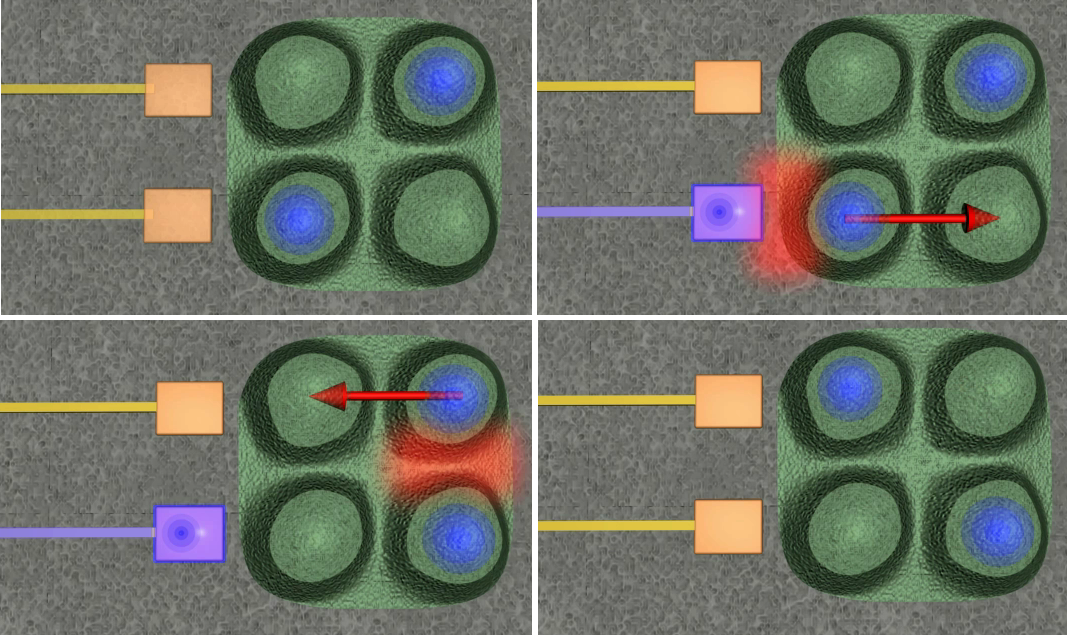
\includegraphics[width=0.8\textwidth]{img/qcaevo.png}}
	\caption{The evolution of the state of a QCA cell. From left to right, from top to bottom: the lower of the two metallic wires (on the left in every image) is polarized, inducing (second image) the lower left electron to flow to the rightmost lower side of the QCA (and precisely inside the corresponding well). This, in turn, induces the upper right electron to move farthest from it, inside the upper left well (third and fourth image).}
	\label{fig:qcaevo}
\end{figure}

An example of a QCA cells based circuit it is reported in Figure \ref{fig:qcaports}. The conjunction of adjacent electrical fields of the three input drivers results into the polarization of the central cell as \textsl{the opposite} of the majority of them, thus inducing the rightmost cell to polarize \textsl{like} them  (thus the name: Majority Gate). By means of the Majority Gate we can build the AND and the AND ports and, with a slightly more complex structure, the NOT one. Thus, any digital circuit can be reimplemented using this technolgy.

\begin{figure}[h!]
	\begin{center}$
		\begin{array}{cc}
			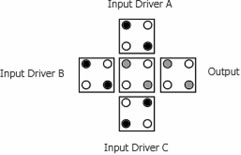
\includegraphics[width=6cm]{img/qcamaj.png} &
			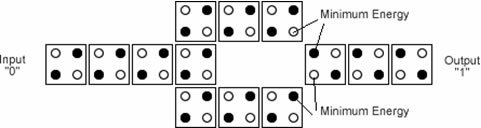
\includegraphics[width=10cm]{img/qcanot.png}
		\end{array}$
	\end{center}
	\caption{\label{fig:qcaports}The majority gate drives the output cell's state to be equal to that of the majority of the inputs. The not port exploit a different angle between cells to obtain the negation of the input.}
\end{figure}


In conclusion, apart from the possibility of using QCA cells for building quantum computers, which is something quite not at hand yet, they can be seen as a powerful alternative to silicon-based devices to represent and transmit data. Depending on the fabrication technique employed, in fact, QCAs are theoretically able to switch at an order of magnitude around the THz, to be packaged at very high density levels and to dissipate very small amounts of power (compared to the current silicon-based technology). This, along with the existance of demo systems already proven working, justifies their current and future development as an attractive way of improving nowadays computing performance bottlenecks.

One of the universities interested and involved into the development of this technology, among the others, is the University of Columbia, and in particular its Microsystems and Nanotechnology Group (MiNa Group). The foundation of our work is their implementation of a simulator (both logical and physical) of QCA based cicuits and it is the subject of the next section.

